\section{Q1: Storm Effect and Model Error}
\label{sec:q1}

\subsection{How much faster do objects fall?}
\label{sec:eventstudy}
Fig.~\ref{fig:es} shows the event study on the main sample (178,107 intervals, 12 clean
storms). Before onset the coefficients wander around zero (placebo pre-trend test $p=0.41$). On day~0 the total
storm effect is about $-30$~m/day and on day~1 about $-12$~m/day. By day~2 it is close to zero,
although days 4 and 5 dip slightly again (about $-5$ and $-7$~m/day). Averaged over days 0--2,
the total storm effect is $-14.1$~m/day (95\% CI $-19.8$ to $-8.4$). Against a pooled quiet-time
mean of about $-50$~m/day, that is roughly 28\% faster decay (Table~\ref{tab:q1}). None of 500
placebo storm dates gives an effect this large ($p<0.002$).

DML tells the same story per unit of storm strength: $\theta = -0.393$~m/day per nT of ap (95\%
CI $-0.527$ to $-0.268$), or $-39$~m/day per 100~nT. A typical day~0 has a mean ap of 57~nT
against a quiet 7~nT, which works out to about $-20$~m/day, in line with the event study. For
$Y_{\text{total}}$, naive regression, linear controls and DML agree to within 1\%. The outcome
already subtracts NRLMSIS run with the real F10.7, so little UV confounding is left. On synthetic data, where UV error goes straight
into the outcome, the naive estimate is biased by more than $+100\%$ and DML is not.

\begin{figure}[t]
\centering
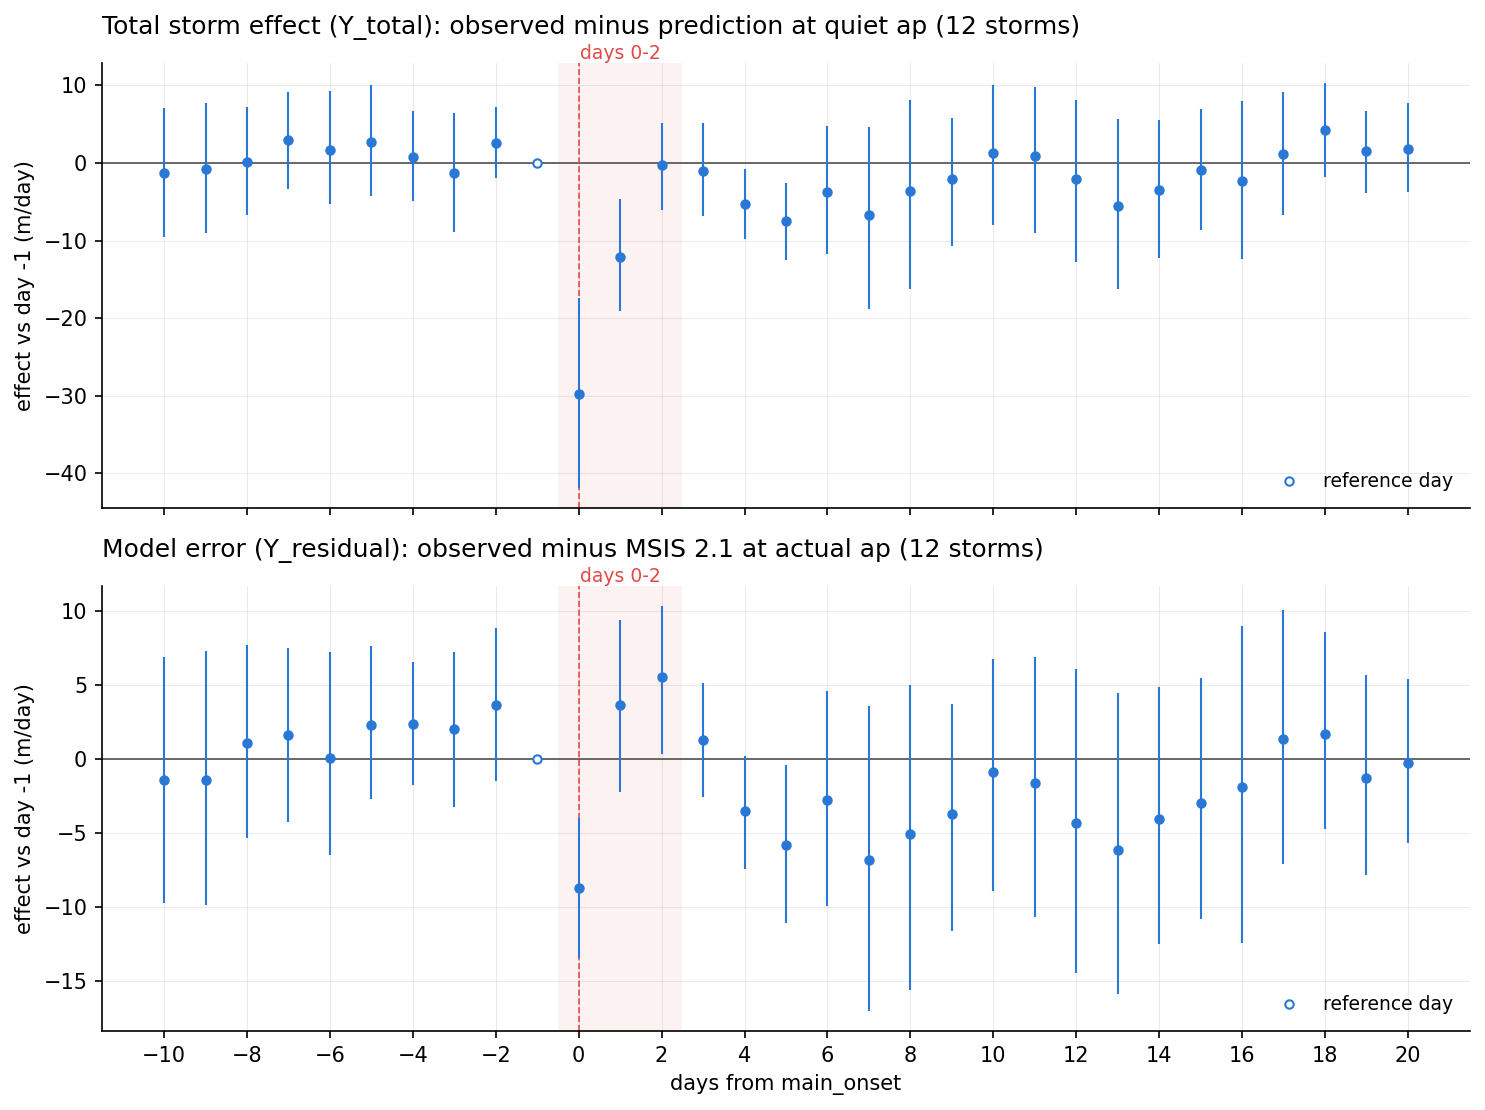
\includegraphics[width=\columnwidth]{fig4_event_study.png}
\caption{Stacked event study (12 clean storms, 95\% storm-clustered intervals). Top: total
storm effect $Y_{\text{total}}$. Bottom: model error $Y_{\text{residual}}$. Day $-1$ is the
reference, and the shaded band marks days 0--2.}
\label{fig:es}
\end{figure}

\begin{table}[t]
\caption{Q1 estimates (m/day; DML in m/day per nT of ap)}
\label{tab:q1}
\centering
\small
\begin{tabular}{@{}lcc@{}}
\toprule
 & $Y_{\text{total}}$ & $Y_{\text{residual}}$ \\
\midrule
Event study, days 0--2 & $-14.1$ & $+0.2$ \\
 & {\scriptsize($-19.8$, $-8.4$)} & {\scriptsize($-3.2$, $+3.2$)} \\
\quad placebo $p$ & $<0.002$ & 0.88 \\
\quad without May/Oct 2024 & $-13.9$ & $-2.2$ \\
 & {\scriptsize($-16.6$, $-10.9$)} & {\scriptsize($-4.4$, $0.0$)} \\
\quad stricter clean rule & $-10.1$ & $+1.4$ \\
 & {\scriptsize($-14.0$, $-6.2$)} & {\scriptsize($-2.5$, $+5.4$)} \\
DML, per nT & $-0.393$ & $-0.050$ \\
 & {\scriptsize($-0.527$, $-0.268$)} & {\scriptsize($-0.141$, $+0.047$)} \\
\quad without May/Oct 2024 & $-0.503$ & $-0.152$ \\
 & {\scriptsize($-0.642$, $-0.361$)} & {\scriptsize($-0.267$, $-0.042$)} \\
\bottomrule
\end{tabular}
\end{table}

The result does not lean on the two biggest storms. Without May and October 2024 the event study
gives $-13.9$~m/day, and DML per nT is actually larger ($-0.503$). Per nT, the total effect is
similar in moderate, strong and severe storms (about $-0.6$~m/day per nT) and smaller in the
single extreme storm (about $-0.25$). That hints at saturation, but with only three large storms
the difference is not significant at the storm level (permutation $p=0.45$).

\subsection{Is NRLMSIS 2.1 wrong during storms?}
\label{sec:modelerror}
On average, not by much, but the average hides a timing problem. Pooled over days 0--2 the
event-study model error is $+0.2$~m/day (95\% CI $-3.2$ to $+3.2$), and the change in the
residual from days $-10..-3$ to days $0..3$, averaged over all 20 storms, is $+0.8$~m/day (CI
$-5.8$ to $+7.4$). Look at Fig.~\ref{fig:es} (bottom), though, and there is a negative error of
about $-9$~m/day on day~0, balanced by small positive errors on days 1--2. DML by storm class
pins this down. In moderate storms the model error is $-0.133$~m/day per nT (95\% CI $-0.247$
to $-0.010$), and in strong storms $-0.210$ (CI $-0.348$ to $-0.068$). In other words, at peak
ap objects lose more altitude than NRLMSIS~2.1 predicts.

There is also a hint of the opposite error a little later. A positive model error 12--24~h after
high ap (24~h lag: $+0.117$, CI $0.035$ to $0.200$) would mean the model keeps the storm
atmosphere around for too long. But it disappears once May and October 2024 are removed (24~h:
$+0.048$, CI $-0.055$ to $+0.152$), so we do not claim it as a general result.

\subsection{The three largest storms}
\label{sec:extreme}
The severe and extreme storms each went wrong in their own way (Fig.~\ref{fig:extreme}).

\textit{October 2024} (severe) is a real model overshoot. The days 0--3 over-prediction survives
3-day smoothing ($+28.4$~m/day, CI $+22.8$ to $+33.9$). From calm day to calm day, objects lost
only 0.86 (CI 0.84--0.87) of the predicted altitude, or $+169$~m once the model's local quiet
error is removed, and this holds in every 100-km band (0.85--0.90).

\textit{May 2024} (extreme) looks like a timing error rather than a wrong total. The early excess
survives smoothing ($+6.9$~m/day), but the calm-to-calm loss is not over-predicted. Against the
model's local quiet error ($\pm30$ days) the difference is $-1$~m (CI $-10$ to $+7$), and against
its pre-storm error the model actually under-predicts the loss by 75~m (CI 59 to 92). So the
model put about the right total, or slightly too little, on the wrong days. The raw ratio of 0.91
comes from an over-prediction that was already there before the storm began.

\textit{December 2024} (severe) goes the other way. Objects lost 1.19 (CI 1.17--1.22) times the
predicted altitude, so here the model under-predicts.

Moving the calm day after the storm two or three days later changes these ratios by at most
0.02, and the high-altitude control differs from its prediction by at most 7~m. So in October and
December the NRLMSIS~2.1 error is 14--19\% of the total calm-to-calm loss (storm plus background
decay), in May it is close to zero once the quiet error is removed, and its sign changes from
storm to storm. No single correction factor would fix all three.

\begin{figure*}[t]
\centering
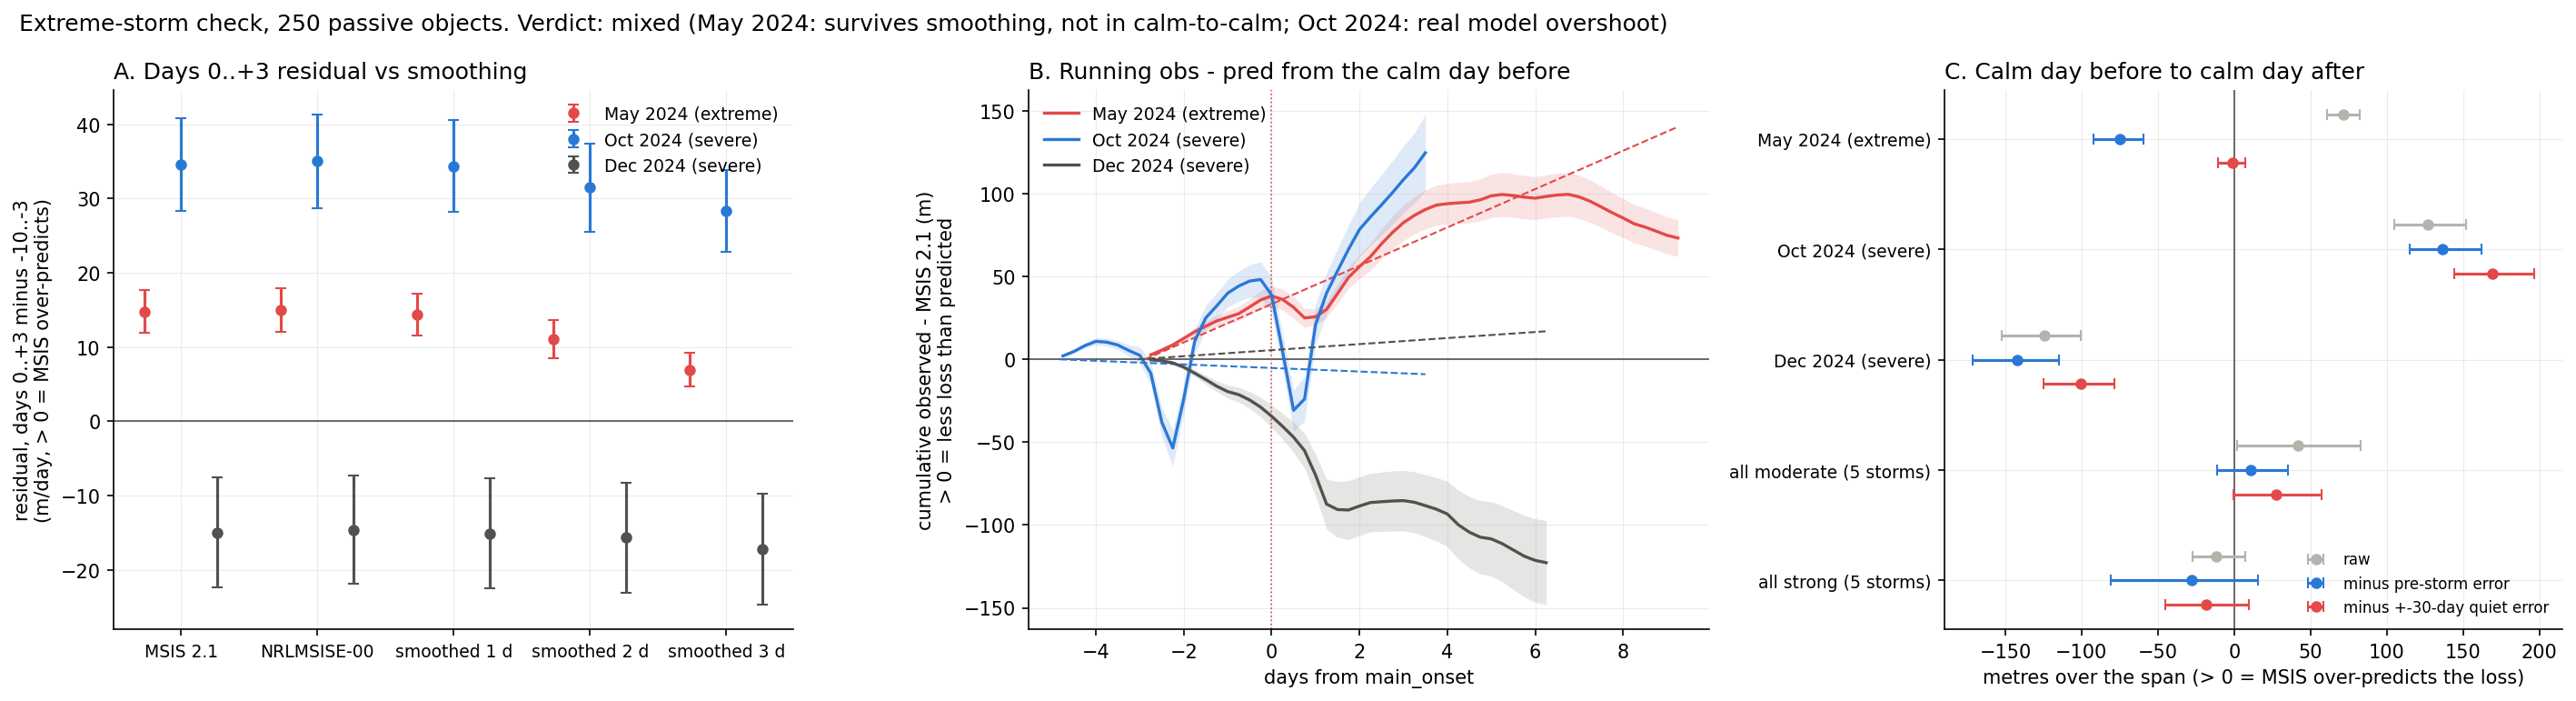
\includegraphics[width=\textwidth]{fig8_extreme_check.png}
\caption{The three largest storms (250 passive objects). (A) Days 0--3 residual change, raw and
smoothed over three days. (B) Running observed minus predicted altitude loss from the calm day
before; dashed: the pre-storm error carried forward. (C) Calm-to-calm loss, observed over
predicted: May 0.91, October 0.86, December 1.19.}
\label{fig:extreme}
\end{figure*}
